\documentclass{article}\usepackage[]{graphicx}\usepackage[]{color}
%% maxwidth is the original width if it is less than linewidth
%% otherwise use linewidth (to make sure the graphics do not exceed the margin)
\makeatletter
\def\maxwidth{ %
  \ifdim\Gin@nat@width>\linewidth
    \linewidth
  \else
    \Gin@nat@width
  \fi
}
\makeatother

\definecolor{fgcolor}{rgb}{0.345, 0.345, 0.345}
\newcommand{\hlnum}[1]{\textcolor[rgb]{0.686,0.059,0.569}{#1}}%
\newcommand{\hlstr}[1]{\textcolor[rgb]{0.192,0.494,0.8}{#1}}%
\newcommand{\hlcom}[1]{\textcolor[rgb]{0.678,0.584,0.686}{\textit{#1}}}%
\newcommand{\hlopt}[1]{\textcolor[rgb]{0,0,0}{#1}}%
\newcommand{\hlstd}[1]{\textcolor[rgb]{0.345,0.345,0.345}{#1}}%
\newcommand{\hlkwa}[1]{\textcolor[rgb]{0.161,0.373,0.58}{\textbf{#1}}}%
\newcommand{\hlkwb}[1]{\textcolor[rgb]{0.69,0.353,0.396}{#1}}%
\newcommand{\hlkwc}[1]{\textcolor[rgb]{0.333,0.667,0.333}{#1}}%
\newcommand{\hlkwd}[1]{\textcolor[rgb]{0.737,0.353,0.396}{\textbf{#1}}}%
\let\hlipl\hlkwb

\usepackage{framed}
\makeatletter
\newenvironment{kframe}{%
 \def\at@end@of@kframe{}%
 \ifinner\ifhmode%
  \def\at@end@of@kframe{\end{minipage}}%
  \begin{minipage}{\columnwidth}%
 \fi\fi%
 \def\FrameCommand##1{\hskip\@totalleftmargin \hskip-\fboxsep
 \colorbox{shadecolor}{##1}\hskip-\fboxsep
     % There is no \\@totalrightmargin, so:
     \hskip-\linewidth \hskip-\@totalleftmargin \hskip\columnwidth}%
 \MakeFramed {\advance\hsize-\width
   \@totalleftmargin\z@ \linewidth\hsize
   \@setminipage}}%
 {\par\unskip\endMakeFramed%
 \at@end@of@kframe}
\makeatother

\definecolor{shadecolor}{rgb}{.97, .97, .97}
\definecolor{messagecolor}{rgb}{0, 0, 0}
\definecolor{warningcolor}{rgb}{1, 0, 1}
\definecolor{errorcolor}{rgb}{1, 0, 0}
\newenvironment{knitrout}{}{} % an empty environment to be redefined in TeX

\usepackage{alltt}
% \usepackage[sc]{mathpazo}
\usepackage{mathptmx}
\usepackage[T1]{fontenc}
\usepackage{geometry}
% \geometry{verbose,tmargin=2.5cm,bmargin=2.5cm,lmargin=2.5cm,rmargin=2.5cm}
\geometry{verbose,tmargin=3.5cm,bmargin=3.5cm,lmargin=3.5cm,rmargin=3.5cm}
\setcounter{secnumdepth}{2}
\setcounter{tocdepth}{2}
\usepackage{url}
\usepackage[unicode=true,pdfusetitle,
bookmarks=true,bookmarksnumbered=true,bookmarksopen=true,bookmarksopenlevel=2,
breaklinks=false,pdfborder={0 0 1},backref=false,colorlinks=true]
{hyperref}
\hypersetup{
  pdfstartview={XYZ null null 1}}
\usepackage{breakurl}
\usepackage{dcolumn}
\usepackage{booktabs}
\usepackage[table]{xcolor}
\usepackage{longtable}
\usepackage{array}
\usepackage{multirow}
\usepackage{wrapfig}
\usepackage{float}
\usepackage{colortbl}
\usepackage{pdflscape}
\usepackage{tabu}
\usepackage{threeparttable}
\usepackage[normalem]{ulem}
\IfFileExists{upquote.sty}{\usepackage{upquote}}{}
\begin{document}



\title{Subtype-Aware Batch Correction Retains Biological Signal\\
  of Integrated Breast Cancer Datasets}

\author{Gil Tom\'as\\
  \href{mailto:gil.tomas@igmm.ed.ac.uk}{gil.tomas@igmm.ed.ac.uk}
}

\maketitle

\tableofcontents







\section{Dataset Acquisition}
\label{sec:acquisition}

Raw CEL files from ten breast cancer gene expression datasets where downloaded
from \href{https://www.ncbi.nlm.nih.gov/geo/}{GEO} and normalized with
\href{https://bioconductor.org/packages/release/bioc/html/frma.html}{fRMA},
\href{https://www.bioconductor.org/packages/release/bioc/html/oligo.html}{RMA}
and
\href{https://www.bioconductor.org/packages/release/bioc/html/affy.html}{MAS5}.
Demographics of each dataset are shown in Table~\ref{tab:demographics}.



\rowcolors{2}{gray!6}{white}
\begin{table}

\caption{\label{tab:demographics}Demographics of datasets in this study.}
\centering
\begin{tabular}[t]{llrrr}
\hiderowcolors
\toprule
GSE & platform & nSamples & fracER+ & fracHER2+\\
\midrule
\showrowcolors
GSE5327 & HG-U133A & 58 & 0.00 & ---\\
GSE25065 & HG-U133A & 198 & 0.62 & 0.01\\
GSE2034 & HG-U133A & 286 & 0.73 & ---\\
GSE17705 & HG-U133A & 298 & 1.00 & ---\\
GSE16446 & HG-U133Plus2 & 120 & 0.00 & 0.33\\
GSE17907 & HG-U133Plus2 & 33 & 0.47 & 1.00\\
GSE21653 & HG-U133Plus2 & 266 & 0.57 & 0.12\\
GSE5460 & HG-U133Plus2 & 127 & 0.58 & 0.24\\
GSE2109 & HG-U133Plus2 & 353 & 0.65 & 0.27\\
GSE23177 & HG-U133Plus2 & 116 & 1.00 & 0.00\\
\bottomrule
\end{tabular}
\end{table}
\rowcolors{2}{white}{white}





\section{Micorarray Dataset Integration}
\label{sec:integration}
Microarray dataset integration needs to account for technical, non-biological,
variation across multiple batches of independently acquired datasets.  The goal
of conventional batch correction (\textsc{bc}) is to remove batch effects while
retaining biological variation conveyed by each dataset.  Several methods exist
to address this task.  One popular approach is
\href{https://www.bu.edu/jlab/wp-assets/ComBat/Abstract.html}{\textsf{ComBat}},
which proposes ``parametric and nonparametric empirical Bayes frameworks for
adjusting data for batch effects that is robust to outliers in small sample
sizes and performs comparable to existing methods for large samples''.  However,
most \textsc{bc} integration strategies do not account for imbalanced subtype
composition within datasets.

This manuscript introduces a novel procedure for integrating expression profile
datasets of known dissimilar composition, called \emph{subtype-aware batch
  correction} (\textsc{sabc}).  Molecular subtypes are initially assigned to
each sample in each dataset with a publicly available single sample predictor
(\textsc{ssp}).  Then, batch effects are resolved between datasets on a
per-subtype basis.  This two-layered approach allows for the biological
specifics captured by the single sample predictor of choice to be accounted for
during the batch correction step, and thus carried over into the integrated
dataset.  By ignoring distinct subtype compositions between datasets,
conventional \textsc{bc} incorrectly apprehends biological variation as
technical batch effect, and consequently distorts true biological signal in the
integrated dataset.

\textsc{sabc} still requires a methodology to address batch effects; we chose
\textsf{ComBat} for this task.  Due to the split of samples by subtype prior to
integration, some subtype-scpecific batches may not have enough samples to draw
summary statistics from; or all samples of a lower frequency subtype may only be
present in one given batch.  Samples that fall in these categories are not
considered (removed from the analysis) by \textsc{sabc}.

Breast cancer is widely understood to be subdivided into five intrinsic or
molecular subtypes, which can be assigned by gene expression profile single
sample predictors.  Breast cancer hence provides an ideal case study for the
evaluation of \textsc{sabc}.  We used conventional \textsc{bc} and \textsc{sabc}
to integrate four breast cancer datasets hybridized onto the \textsf{Affymetrix}
HG-U133a chip and six breast cancer datasets hybridized onto the
HG-U133Plus2 chip (Table \ref{tab:demographics}).


To evaluate the performance of each method, we compared the distributions of
expression values for the
\href{https://genecards.weizmann.ac.il/cgi-bin/geneannot/GA_search.pl?keyword_type=probe_set_id&array=HG-U133&target=genecards&keyword=205225_at}{205225\_at}
and the
\href{https://genecards.weizmann.ac.il/cgi-bin/geneannot/GA_search.pl?keyword_type=probe_set_id&array=HG-U133&target=genecards&keyword=216836_s_at}{216836\_s\_at}
probesets in each chip, respectively targeting for the \emph{ESR1} and
\emph{ERBB2} gene transcripts.  Estrogen receptor (\textsc{esr1}) and
Erb-B2 Receptor Tyrosine Kinase 2 receptor (\textsc{erbb2}) status are strong
predictors of breast cancer prognosis and are traditionally assessed by
immunohistochemestry (\textsc{ihc}).  Post dataset integration, the expression
values of both genes should remain in line with the biological signal conveyed
by the independent assessment given by \textsc{ihc} for both proteins.  In
addition, we compared the agreement between single sample predictor class
assignments for individual samples prior and post integration.  The batch
correction procedure should not interfere with the molecular subtype identity of
each sample, and for that reason higher agreement rates should be indicative of
higher transcriptional fidelity of the integrated dataset.

To guide the integration process with \textsc{sabc}, we used two \textsc{ssp}s
implemented in the
\href{https://bioconductor.org/packages/release/bioc/html/genefu.html}{\textsf{Genefu}}
Bioconductor package.  The first,
\href{http://www.pnas.org/content/100/14/8418}{\textsf{sorlie2003}}, is based on
534 diagnostic genes and is a five-subtype classifier; the second,
\href{http://clincancerres.aacrjournals.org/content/14/16/5158?ck=nck}{\textsf{desmedt2008}},
is based on three genes (\emph{ESR1}, \emph{ERBB2} and \emph{AURKA}), and is a
three-subtype classifier.  To assess classifier agreement prior and post
integration, and in order to circumvent the redundancy caused by using the same
single sample predictor to integrate and to validate the integration process, we
used the Genefu implementation of the
\href{http://ascopubs.org/doi/abs/10.1200/JCO.2008.18.1370}{\textsc{pam50}}
single sample predictor, based on 50 genes and yielding a five-subtype
classifier.

\subsection{Prior \textsc{ssp} predictions}
\label{sec:preds}

Prior to datset integration with \textsc{sabc}, we compute \textsc{ssp} classes
for each dataset in our analysis.  Tables~\ref{tab:tab-desmedt2008}
and~\ref{tab:tab-sorlie2003} respectively show the partitions of each of the 3-
and 5-class \textsc{ssp}s across the four HG-U133a datasets in this study.  We
then computed \textsc{ssp} predictions for both the \textsf{desmedt2008} and
\textsf{sorlie2003} classifier in each integrated expression matrix.



\rowcolors{2}{gray!6}{white}
\begin{table}

\caption{\label{tab:tab-desmedt2008}Partition of desmedt2008 subtypes in the ten datasets in this study (fRMA normalization).}
\centering
\begin{tabular}[t]{lrrr}
\hiderowcolors
\toprule
  & ER-/HER2- & ER+/HER2- & HER2+\\
\midrule
\showrowcolors
\addlinespace[0.3em]
\multicolumn{4}{l}{\textbf{HG-U133a}}\\
\hspace{1em}GSE5327 & 37 & 13 & 8\\
\hspace{1em}GSE25065 & 75 & 93 & 30\\
\hspace{1em}GSE2034 & 61 & 189 & 36\\
\hspace{1em}GSE17705 & 54 & 218 & 26\\
\addlinespace[0.3em]
\multicolumn{4}{l}{\textbf{HG-U133Plus2}}\\
\hspace{1em}GSE16446 & 77 & 19 & 24\\
\hspace{1em}GSE17907 & 6 & 15 & 12\\
\hspace{1em}GSE21653 & 75 & 149 & 42\\
\hspace{1em}GSE5460 & 35 & 74 & 18\\
\hspace{1em}GSE2109 & 97 & 210 & 46\\
\hspace{1em}GSE23177 & 15 & 78 & 23\\
\bottomrule
\end{tabular}
\end{table}
\rowcolors{2}{white}{white}



\rowcolors{2}{gray!6}{white}
\begin{table}

\caption{\label{tab:tab-sorlie2003}Partition of sorlie2003 subtypes in the ten datasets in this study (fRMA normalization).}
\centering
\begin{tabular}[t]{lrrrrr}
\hiderowcolors
\toprule
  & Basal & Her2 & LumA & LumB & Normal\\
\midrule
\showrowcolors
\addlinespace[0.3em]
\multicolumn{6}{l}{\textbf{HG-U133a}}\\
\hspace{1em}GSE5327 & 32 & --- & 1 & 25 & ---\\
\hspace{1em}GSE25065 & 48 & --- & 39 & 108 & 3\\
\hspace{1em}GSE2034 & 48 & 1 & 84 & 152 & 1\\
\hspace{1em}GSE17705 & 6 & --- & 144 & 140 & 8\\
\addlinespace[0.3em]
\multicolumn{6}{l}{\textbf{HG-U133Plus2}}\\
\hspace{1em}GSE16446 & 68 & 1 & 1 & 50 & ---\\
\hspace{1em}GSE17907 & 2 & 4 & 3 & 23 & 1\\
\hspace{1em}GSE21653 & 68 & 7 & 89 & 95 & 7\\
\hspace{1em}GSE5460 & 32 & --- & 47 & 48 & ---\\
\hspace{1em}GSE2109 & 65 & 5 & 128 & 144 & 11\\
\hspace{1em}GSE23177 & 2 & --- & 33 & 81 & ---\\
\bottomrule
\end{tabular}
\end{table}
\rowcolors{2}{white}{white}



\subsection{Integration}
\label{sec:integrate}
Integrated matrices of gene expression were computed for each normalization
method (f\textsc{rma}, \textsc{rma} and \textsc{mas5}) and each integration
method (\textsc{bc} and \textsc{sabc}, driven by 3- and 5-subtype classifier).





\section{Comparison of Integration Methods}
\label{sec:evaluation}

\subsection{Distortion of Molecular \emph{ESR1} measurements}
\label{sec:distortion-ESR1}
We compared the distributions of expression values prior and post dataset
integration for the \textsf{205225\_at} probeset in 840 breast tumours,
hybridized onto the HG-U133a chip, from four datasets with distinct fractions of
ER$+$ samples (Table~\ref{tab:demographics} and Figure~\ref{fig:er-a-boxplots}).
Regardless of the normalization method, \textsc{bc} integration significantly
distorts \emph{ESR1} expression measurements in samples from datasets with
extreme fractions of ER$+$ samples (GSE5327 and GSE17705), to the point where
the two distributions no longer can tell the difference between ER$-$ and ER$+$
samples (Figure~\ref{fig:er-a-extreme-datasets-by-er-status}, second column of
panels).  In both cases, \textsc{sabc} integration, whether driven by a
3-subtype \textsc{ssp} (\textsc{sabc3}) or a 5-subtype \textsc{ssp}
(\textsc{sabc5}), succeeds in retaining the biological signal conveyed by the
IHC status in datasets with extreme compositions
(Figure~\ref{fig:er-a-extreme-datasets-by-er-status}, third and fourth columns
of panels).  Further comparison of ESR1 transcript abundance in these two
datasets prior and post integration reveals that expression values depart
significantly from original measurements when datasets are integrated with
\textsc{bc}, yet are preserved from extreme distortion by \textsc{sabc}
integration (Figure~\ref{fig:er-a-extreme-datasets-by-integration}).



\begin{knitrout}
\definecolor{shadecolor}{rgb}{0.969, 0.969, 0.969}\color{fgcolor}\begin{figure}

{\centering 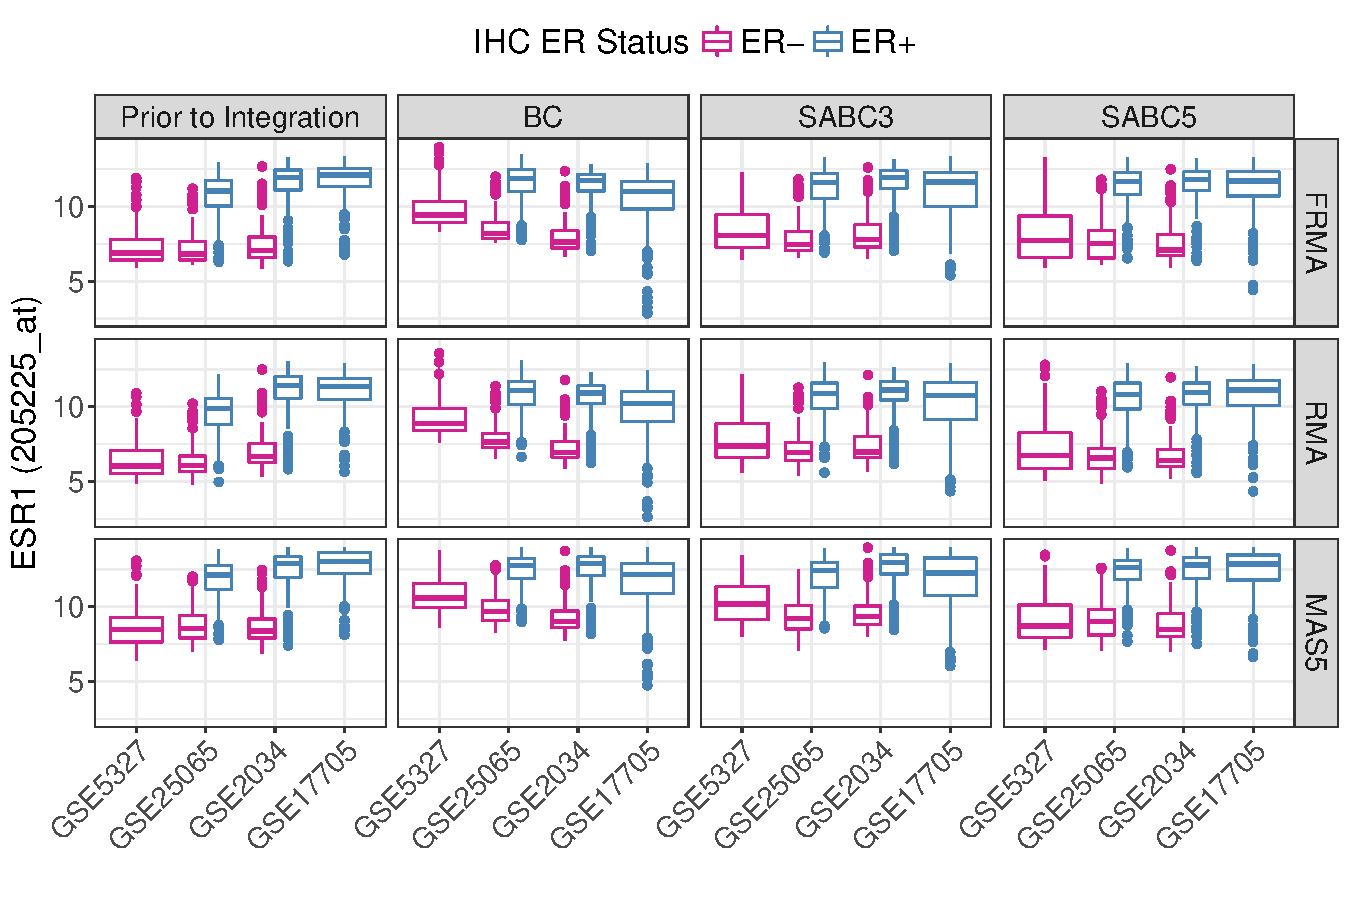
\includegraphics[width=\maxwidth]{figure/er-a-boxplots-1} 

}

\caption[20225\_at probeset measurements hybridized onto the HG-U133a chip broken by dataset prior and post integration]{20225\_at probeset measurements hybridized onto the HG-U133a chip broken by dataset prior and post integration.  Integration was done using standard batch correction (BC, with ComBat) and subtype-aware batch correction (SABC3, driven by a three-subtype SSP---desmedt2008; and SABC5, driven by a five-subtype SSP---sorlie2003).  The distributions are further split by ER status, independently assessed by IHC on fresh frozen specimens.  Raw data was normalised with FRMA, RMA and MAS5.}\label{fig:er-a-boxplots}
\end{figure}


\end{knitrout}

\begin{knitrout}
\definecolor{shadecolor}{rgb}{0.969, 0.969, 0.969}\color{fgcolor}\begin{figure}

{\centering 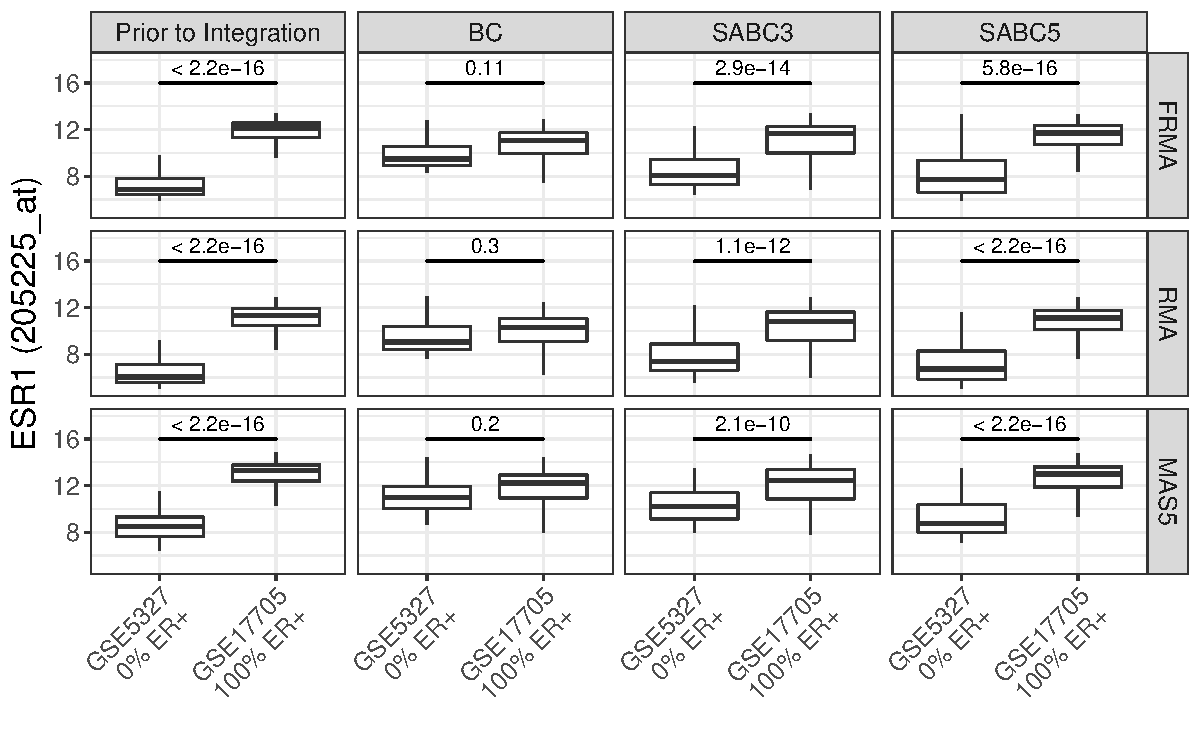
\includegraphics[width=\maxwidth]{figure/er-a-extreme-datasets-by-er-status-1} 

}

\caption[Distributions of probeset 205225\_at measurements from datasets GSE5327 (n=58, all ER-) and GSE17705 (n=298, all ER+), taken from Figure 1, are compared side by side]{Distributions of probeset 205225\_at measurements from datasets GSE5327 (n=58, all ER-) and GSE17705 (n=298, all ER+), taken from Figure 1, are compared side by side. See Figure 1 for details.}\label{fig:er-a-extreme-datasets-by-er-status}
\end{figure}


\end{knitrout}

\begin{knitrout}
\definecolor{shadecolor}{rgb}{0.969, 0.969, 0.969}\color{fgcolor}\begin{figure}

{\centering 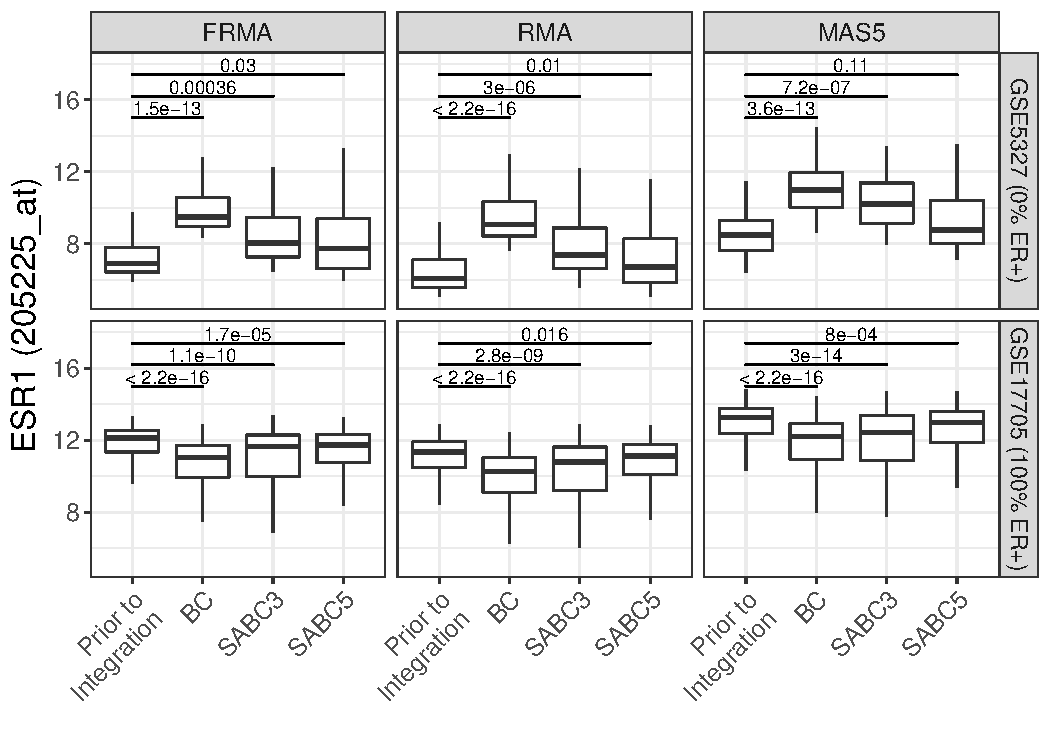
\includegraphics[width=\maxwidth]{figure/er-a-extreme-datasets-by-integration-1} 

}

\caption[Distributions of probeset 205225\_at measurements from datasets GSE5327 (n=58, all ER-) and GSE17705 (n=298, all ER+), taken from Figure 1, are each compared prior and post dataset integration]{Distributions of probeset 205225\_at measurements from datasets GSE5327 (n=58, all ER-) and GSE17705 (n=298, all ER+), taken from Figure 1, are each compared prior and post dataset integration.  See Figure 1 for details.}\label{fig:er-a-extreme-datasets-by-integration}
\end{figure}


\end{knitrout}

\subsection{Distortion of Molecular \emph{ERBB2} measurements}
\label{sec:distortion-ERBB2}

Although less pronounced, a similar trend is observed when comparing the
expression values prior and post- dataset integration for the
\textsf{216836\_s\_at} probeset, in 1015 breast tumours hybridized onto the
HG-U133Plus2 chip, from six datasets with distinct proportions of HER2+ samples
(Table~\ref{tab:demographics} and
Figure~\ref{fig:her2-p2-extreme-datasets-by-her-status}).  Regardless of the
normalisation protocol, The ERBB2 probeset distributions clearly reflect the IHC
HER2 receptor status in the two datasets in our analysis with extreme HER2
compositions (GSE23177, all HER2--; and GSE17907, all HER2+).  When the five
datasets are integrated with \textsc{bc}, this biological signal is erased, yet
preserved (albeit to a lesser extent than in the original datasets), when
integrated with \textsc{sabc3} and \textsc{sabc5}
(Figure~\ref{fig:her2-p2-extreme-datasets-by-her-status}).

The different degree to which subtype-aware batch correction successfully
retains biological signal from these two molecular correlates of breast cancer
biology, in datasets with extreme compositions, could be explained by how well
the classifiers used to drive integration capture the underlying biology of the
ER and HER2 receptors.  Because the clinical HER2 breast cancer phenotype is the
result of a gene amplification, it is possible that gene expression classifiers
are less apt to model binary gene expression distributions (HER2) rather than
continuous ones (ER).  In addition, the top level split highlighted by most
molecular characterisations of breast tumours is lead by ER status, consigning
most \textsc{ssp} derived from molecular data to be particularly sensitive to
biological signal conveyed by this marker.

\begin{knitrout}
\definecolor{shadecolor}{rgb}{0.969, 0.969, 0.969}\color{fgcolor}\begin{figure}

{\centering 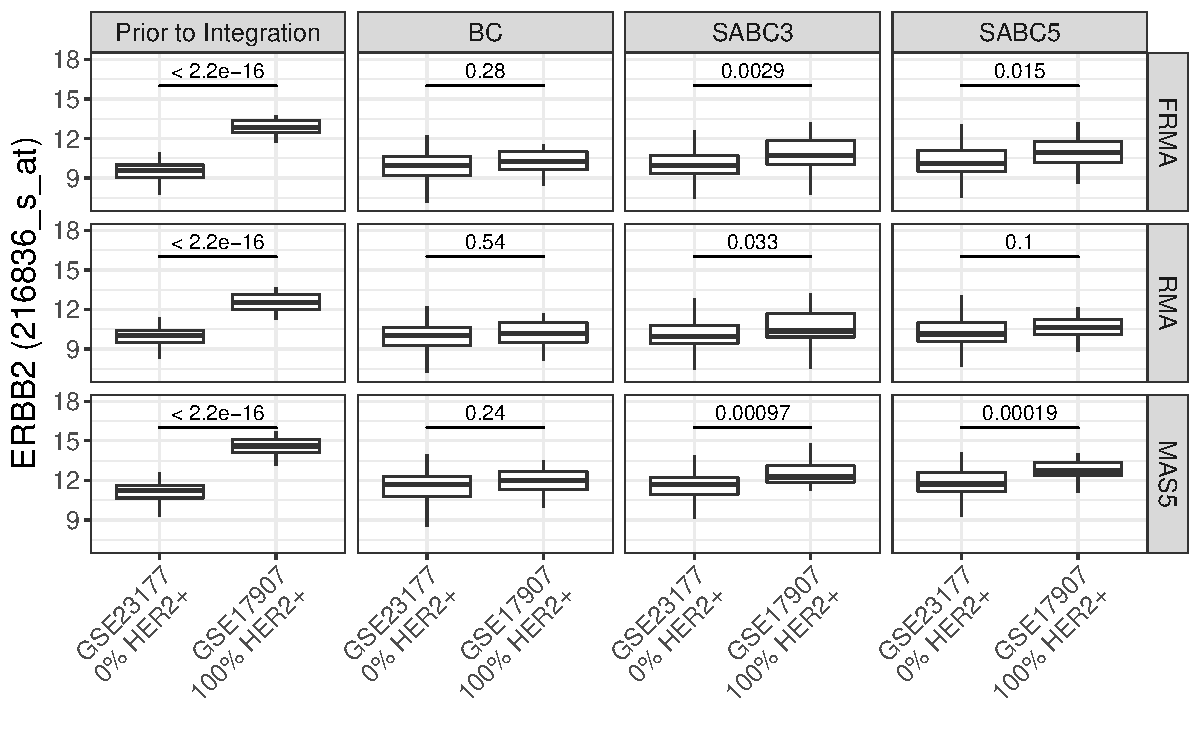
\includegraphics[width=\maxwidth]{figure/her2-p2-extreme-datasets-by-her-status-1} 

}

\caption[216836\_s\_at probeset measurements hybridized onto the HG-U133Plus2 chip are shown for datasets GSE23177 (n=116, all HER2-) and GSE17907 (n=37, all HER2+), in the leftmost column]{216836\_s\_at probeset measurements hybridized onto the HG-U133Plus2 chip are shown for datasets GSE23177 (n=116, all HER2-) and GSE17907 (n=37, all HER2+), in the leftmost column.  These two datasets were integrated with GSE16446, GSE21653, GSE5460 and GSE2109 (Table 1), with BC, SABC3 and SABC5.  ERBB2 expression values for the samples in the two datasets with extreme HER2+ compositions are then shown post-integration with each of these methods, broken by normalisation procedure (cf. Figure 1 for more details).}\label{fig:her2-p2-extreme-datasets-by-her-status}
\end{figure}


\end{knitrout}

\subsection{Single Sample Predictor Agreement}
\label{sec:concordance}

Single sample predictor assignments for the Genefu implementation of the
\textsc{pam50} breast cancer classifier were computed for each of the 1015
samples in GSE2109, GSE21653, GSE5460, GSE16446, GSE23177 and GSE17907, after
f\textsc{rma} normalization (Table~\ref{tab:demographics}).  We then integrated
the six datasets with \textsc{bc}, \textsc{sabc3} and \textsc{sabc5}, and
computed each sample's \textsc{pam50} subtype post-integration.  Comparisons of
subtype assignments prior- and post-integration can be seen in
Figure~\ref{fig:pam50-concordance-plot} and in Table~\ref{tab:tab-p2-kvals}.

With the exception of the largest dataset, GSE2109, \textsc{pam50} interrater
agreement was always higher with \textsc{sabc} integration than with
conventional integration.  Incidentally, the datasets that showed lesser subtype
agreement post \textsc{bc} integration are the ones with most extreme ER and
HER2 compositions (GSE16446, GSE23177 and GSE17907).  For these datasets,
\textsc{sabc} integration was able to increase subtype assignment agreement
(with the exception of \textsc{sabc3} for GSE23177).





\begin{knitrout}
\definecolor{shadecolor}{rgb}{0.969, 0.969, 0.969}\color{fgcolor}\begin{figure}

{\centering 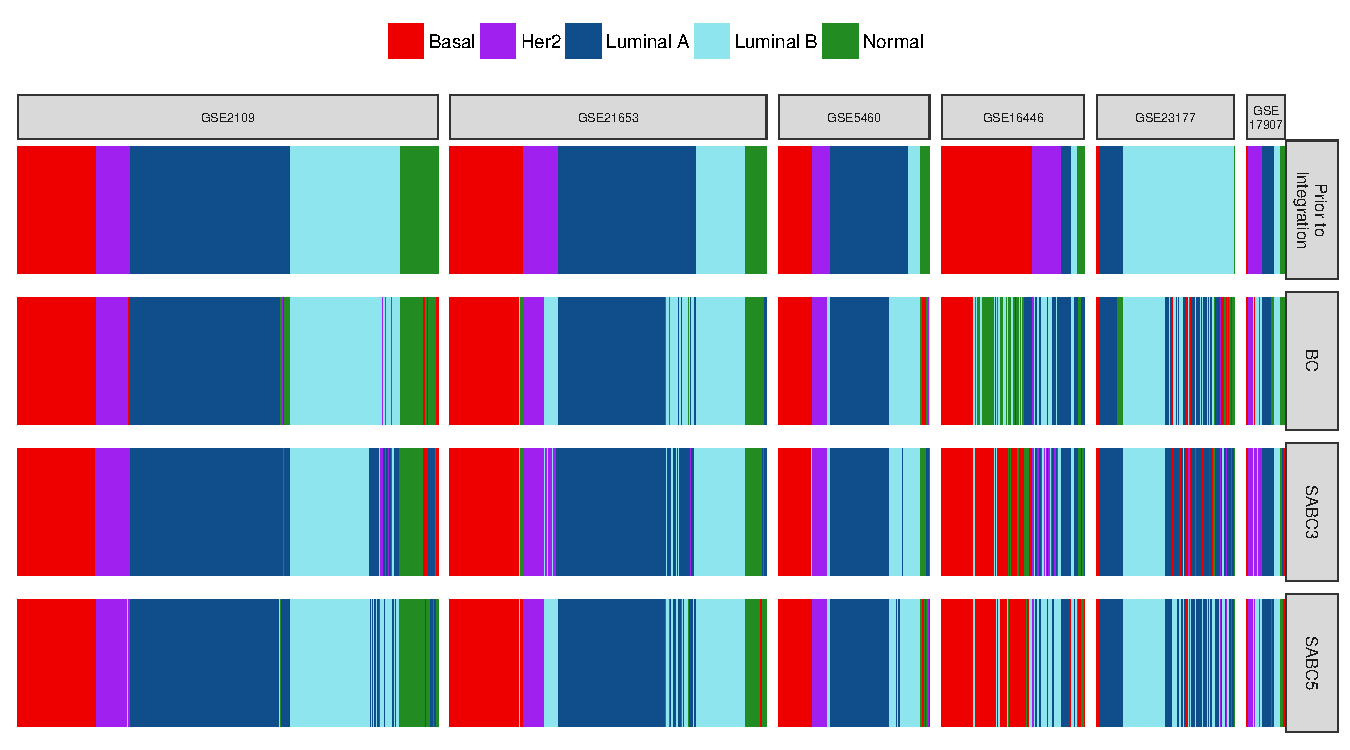
\includegraphics[width=\maxwidth]{figure/pam50-concordance-plot-1} 

}

\caption[PAM50 subtype assignments for 1015 samples from six datasets (Table 1) hybridized on the HG-U133Plus2 chip and normalized with FRMA]{PAM50 subtype assignments for 1015 samples from six datasets (Table 1) hybridized on the HG-U133Plus2 chip and normalized with FRMA.  Subtype assignements were computed prior to dataset integration (first row) and post integration with BC, SABC3 and SABC5 (subsequent rows).}\label{fig:pam50-concordance-plot}
\end{figure}


\end{knitrout}



\rowcolors{2}{gray!6}{white}
\begin{table}

\caption{\label{tab:tab-p2-kvals}Interrater agreement of PAM50 subtype assignment prior- and post-dataset integration (see text for details).}
\centering
\begin{tabular}[t]{lrrrrrrr}
\hiderowcolors
\toprule
  & all & GSE2109 & GSE21653 & GSE5460 & GSE16446 & GSE23177 & GSE17907\\
\midrule
\showrowcolors
\addlinespace[0.3em]
\multicolumn{8}{l}{\textbf{Clinical}}\\
\hspace{1em}nSamples & 1015 & 353 & 266 & 127 & 120 & 116 & 33\\
\hspace{1em}\% ER+ & --- & 65 & 57 & 58 & 0 & 100 & 47\\
\hspace{1em}\% HER2+ & --- & 27 & 12 & 24 & 33 & 0 & 100\\
\addlinespace[0.3em]
\multicolumn{8}{l}{\textbf{Cohen's Kappa (\%)}}\\
\hspace{1em}BC & 72 & 95 & 80 & 72 & 21 & 30 & 58\\
\hspace{1em}SABC3 & 78 & 85 & 90 & 75 & 63 & 25 & 79\\
\hspace{1em}SABC5 & 80 & 93 & 85 & 76 & 50 & 40 & 61\\
\bottomrule
\end{tabular}
\end{table}
\rowcolors{2}{white}{white}



\subsection{Effect of Sample Size}
\label{sec:size}

Because sample size can further confound the effect of dataset composition
towards retention of biological signal post-integration, we compared the
\textsc{pam50} interrate agreement prior and post-integration for datasets
GSE2109, GSE21653, GSE5460, GSE16446 and GSE23177, sampling, in each dataset, 116
samples with the same IHC ER+ proportions as the original datasets.  Comparisons
of subtype assignements prior and post-integration in this experiment can be
seen in Figure~\ref{fig:pam50-concordance-proportions-plot} and
Table~\ref{tab:tab-p2-kvals-proportions}.  Notice how dataset size normalization
further emphasises the need for subtype-aware batch correction.



\begin{knitrout}
\definecolor{shadecolor}{rgb}{0.969, 0.969, 0.969}\color{fgcolor}\begin{figure}

{\centering 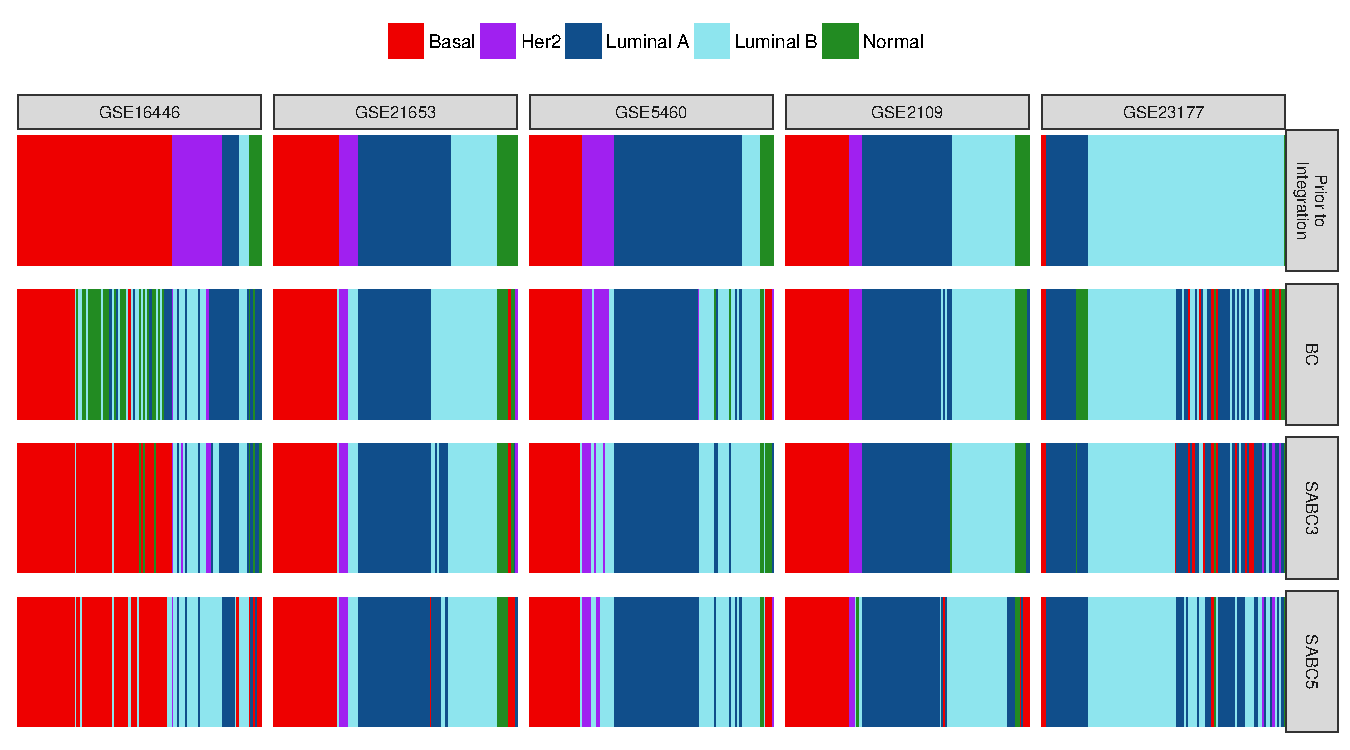
\includegraphics[width=\maxwidth]{figure/pam50-concordance-proportions-plot-1} 

}

\caption[PAM50 subtype assignments for 580 samples from five datasets (Table 1) hybridized on the HG-U133Plus2 chip and normalised with FRMA]{PAM50 subtype assignments for 580 samples from five datasets (Table 1) hybridized on the HG-U133Plus2 chip and normalised with FRMA.  For each dataset, 116 samples were randomly selected in order to respect the original IHC ER+ fraction.  Subtype assignments were computed prior- (top row) and post- (subsequent rows) dataset integration with BC, SABC3 and SABC5}\label{fig:pam50-concordance-proportions-plot}
\end{figure}


\end{knitrout}



\rowcolors{2}{gray!6}{white}
\begin{table}

\caption{\label{tab:tab-p2-kvals-proportions}Interrater agreement of PAM50 subtype assignment prior- and post-dataset integration, when datasets are all brought down to the same size (n = 116, see text for details).}
\centering
\begin{tabular}[t]{lrrrrrr}
\hiderowcolors
\toprule
  & all & GSE16446 & GSE21653 & GSE5460 & GSE2109 & GSE23177\\
\midrule
\showrowcolors
\addlinespace[0.3em]
\multicolumn{7}{l}{\textbf{Clinical}}\\
\hspace{1em}nSamples & 580 & 116 & 116 & 116 & 116 & 116\\
\hspace{1em}\% ER+ & --- & 0 & 57 & 58 & 65 & 100\\
\hspace{1em}\% HER2+ & --- & 33 & 12 & 24 & 27 & 0\\
\addlinespace[0.3em]
\multicolumn{7}{l}{\textbf{Cohen's Kappa (\%)}}\\
\hspace{1em}BC & 62 & 23 & 79 & 69 & 96 & 32\\
\hspace{1em}SABC3 & 71 & 59 & 84 & 65 & 96 & 31\\
\hspace{1em}SABC5 & 69 & 45 & 82 & 63 & 81 & 47\\
\bottomrule
\end{tabular}
\end{table}
\rowcolors{2}{white}{white}



\section{Comparison with Published Methods}
\label{sec:published}

\textsc{sabc} is not the first method to account for external biological
variables or clinical covariates during dataset integration.  ComBat offers the
possibility of using clinical variables as covariates during dataset
integration.  \href{https://www.ncbi.nlm.nih.gov/pubmed/27585881}{Harman}, a
more recent integration procedure using a PCA and a constrained optimisation
technique, also calls for factor coding for an ``experimental grouping
variable'' to drive integration.  We ran Harman to integrate the 840 breast
tumours hybridised onto the the HG-U133a chip (normalized with f\textsc{rma}),
using the the output of the 5-class sorlie2003 SSP as covariate and experimental
grouping variable respectively.  As seen in
Figure~\ref{fig:er-a-boxplots-other}, dataset integration with Harman fails to
retain the original difference in ESR1 measurements prior to integration for
datasets GSE5327 and GSE17705.

\begin{knitrout}
\definecolor{shadecolor}{rgb}{0.969, 0.969, 0.969}\color{fgcolor}\begin{figure}

{\centering 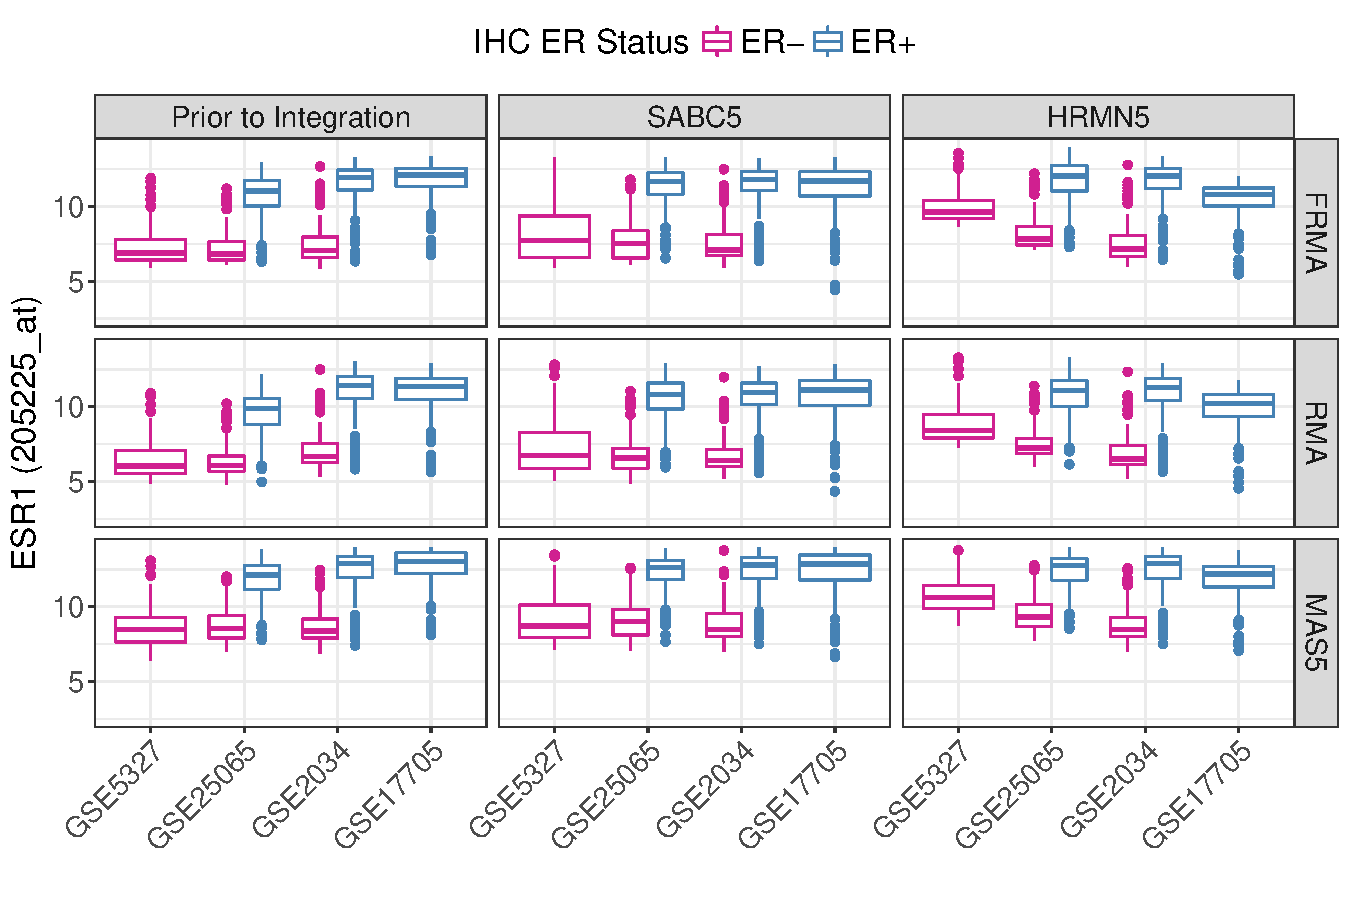
\includegraphics[width=\maxwidth]{figure/er-a-boxplots-other-1} 

}

\caption[205225\_at probeset measurements hybridized onto the HG-U133a chip broken by dataset prior and post integration]{205225\_at probeset measurements hybridized onto the HG-U133a chip broken by dataset prior and post integration.  Integration was done using subtype-aware batch correction (SABC5, driven by a five-subtype SSP) and Harman (HRMN5, using a five-subtype SSP as a grouping variable).  The distributions are further split by ER status, independently assessed by IHC on fresh frozen specimens.  Raw data was normalised with FRMA, RMA and MAS5.}\label{fig:er-a-boxplots-other}
\end{figure}


\end{knitrout}

\end{document}
